\documentclass[conference]{IEEEtran}
\usepackage{blindtext, graphicx}
\usepackage{amsmath}
\usepackage{amsfonts}
\usepackage{listings}
\usepackage{multicol}
\usepackage{lipsum}
\usepackage{color}
\usepackage{todonotes}
\usepackage{cite}
\usepackage[english]{babel}

\lstset{
  language=Python,
  showstringspaces=false,
  formfeed=\newpage,
  tabsize=4,
  commentstyle=\itshape,
  basicstyle=\ttfamily\scriptsize,
  morekeywords={lambda, self, assert, as},
  numbers=none,
  numberstyle=\scriptsize\color{light-gray}\textsf,
  frame=single
}


\DeclareMathOperator*{\argmax}{arg\, max}

% Add the compsoc option for Computer Society conferences.
%
% If IEEEtran.cls has not been installed into the LaTeX system files,
% manually specify the path to it like:
% \documentclass[conference]{../sty/IEEEtran}

% Some very useful LaTeX packages include:
% (uncomment the ones you want to load)


% *** MISC UTILITY PACKAGES ***
%
%\usepackage{ifpdf}
% Heiko Oberdiek's ifpdf.sty is very useful if you need conditional
% compilation based on whether the output is pdf or dvi.
% usage:
% \ifpdf
%   % pdf code
% \else
%   % dvi code
% \fi
% The latest version of ifpdf.sty can be obtained from:
% http://www.ctan.org/tex-archive/macros/latex/contrib/oberdiek/
% Also, note that IEEEtran.cls V1.7 and later provides a builtin
% \ifCLASSINFOpdf conditional that works the same way.
% When switching from latex to pdflatex and vice-versa, the compiler may
% have to be run twice to clear warning/error messages.






% *** CITATION PACKAGES ***
%
%\usepackage{cite}
% cite.sty was written by Donald Arseneau
% V1.6 and later of IEEEtran pre-defines the format of the cite.sty package
% \cite{} output to follow that of IEEE. Loading the cite package will
% result in citation numbers being automatically sorted and properly
% "compressed/ranged". e.g., [1], [9], [2], [7], [5], [6] without using
% cite.sty will become [1], [2], [5]--[7], [9] using cite.sty. cite.sty's
% \cite will automatically add leading space, if needed. Use cite.sty's
% noadjust option (cite.sty V3.8 and later) if you want to turn this off.
% cite.sty is already installed on most LaTeX systems. Be sure and use
% version 4.0 (2003-05-27) and later if using hyperref.sty. cite.sty does
% not currently provide for hyperlinked citations.
% The latest version can be obtained at:
% http://www.ctan.org/tex-archive/macros/latex/contrib/cite/
% The documentation is contained in the cite.sty file itself.






% *** GRAPHICS RELATED PACKAGES ***
%
\graphicspath{{./images/}}
\ifCLASSINFOpdf
  % \usepackage[pdftex]{graphicx}
  % declare the path(s) where your graphic files are
  % \graphicspath{{../pdf/}{../jpeg/}}
  % and their extensions so you won't have to specify these with
  % every instance of \includegraphics
  % \DeclareGraphicsExtensions{.pdf,.jpeg,.png}
\else
  % or other class option (dvipsone, dvipdf, if not using dvips). graphicx
  % will default to the driver specified in the system graphics.cfg if no
  % driver is specified.
  % \usepackage[dvips]{graphicx}
  % declare the path(s) where your graphic files are
  % \graphicspath{{../eps/}}
  % and their extensions so you won't have to specify these with
  % every instance of \includegraphics
  % \DeclareGraphicsExtensions{.eps}
\fi
% graphicx was written by David Carlisle and Sebastian Rahtz. It is
% required if you want graphics, photos, etc. graphicx.sty is already
% installed on most LaTeX systems. The latest version and documentation can
% be obtained at:
% http://www.ctan.org/tex-archive/macros/latex/required/graphics/
% Another good source of documentation is "Using Imported Graphics in
% LaTeX2e" by Keith Reckdahl which can be found as epslatex.ps or
% epslatex.pdf at: http://www.ctan.org/tex-archive/info/
%
% latex, and pdflatex in dvi mode, support graphics in encapsulated
% postscript (.eps) format. pdflatex in pdf mode supports graphics
% in .pdf, .jpeg, .png and .mps (metapost) formats. Users should ensure
% that all non-photo figures use a vector format (.eps, .pdf, .mps) and
% not a bitmapped formats (.jpeg, .png). IEEE frowns on bitmapped formats
% which can result in "jaggedy"/blurry rendering of lines and letters as
% well as large increases in file sizes.
%
% You can find documentation about the pdfTeX application at:
% http://www.tug.org/applications/pdftex





% *** MATH PACKAGES ***
%
%\usepackage[cmex10]{amsmath}
% A popular package from the American Mathematical Society that provides
% many useful and powerful commands for dealing with mathematics. If using
% it, be sure to load this package with the cmex10 option to ensure that
% only type 1 fonts will utilized at all point sizes. Without this option,
% it is possible that some math symbols, particularly those within
% footnotes, will be rendered in bitmap form which will result in a
% document that can not be IEEE Xplore compliant!
%
% Also, note that the amsmath package sets \interdisplaylinepenalty to 10000
% thus preventing page breaks from occurring within multiline equations. Use:
%\interdisplaylinepenalty=2500
% after loading amsmath to restore such page breaks as IEEEtran.cls normally
% does. amsmath.sty is already installed on most LaTeX systems. The latest
% version and documentation can be obtained at:
% http://www.ctan.org/tex-archive/macros/latex/required/amslatex/math/





% *** SPECIALIZED LIST PACKAGES ***
%
%\usepackage{algorithmic}
% algorithmic.sty was written by Peter Williams and Rogerio Brito.
% This package provides an algorithmic environment fo describing algorithms.
% You can use the algorithmic environment in-text or within a figure
% environment to provide for a floating algorithm. Do NOT use the algorithm
% floating environment provided by algorithm.sty (by the same authors) or
% algorithm2e.sty (by Christophe Fiorio) as IEEE does not use dedicated
% algorithm float types and packages that provide these will not provide
% correct IEEE style captions. The latest version and documentation of
% algorithmic.sty can be obtained at:
% http://www.ctan.org/tex-archive/macros/latex/contrib/algorithms/
% There is also a support site at:
% http://algorithms.berlios.de/index.html
% Also of interest may be the (relatively newer and more customizable)
% algorithmicx.sty package by Szasz Janos:
% http://www.ctan.org/tex-archive/macros/latex/contrib/algorithmicx/




% *** ALIGNMENT PACKAGES ***
%
%\usepackage{array}
% Frank Mittelbach's and David Carlisle's array.sty patches and improves
% the standard LaTeX2e array and tabular environments to provide better
% appearance and additional user controls. As the default LaTeX2e table
% generation code is lacking to the point of almost being broken with
% respect to the quality of the end results, all users are strongly
% advised to use an enhanced (at the very least that provided by array.sty)
% set of table tools. array.sty is already installed on most systems. The
% latest version and documentation can be obtained at:
% http://www.ctan.org/tex-archive/macros/latex/required/tools/


%\usepackage{mdwmath}
%\usepackage{mdwtab}
% Also highly recommended is Mark Wooding's extremely powerful MDW tools,
% especially mdwmath.sty and mdwtab.sty which are used to format equations
% and tables, respectively. The MDWtools set is already installed on most
% LaTeX systems. The lastest version and documentation is available at:
% http://www.ctan.org/tex-archive/macros/latex/contrib/mdwtools/


% IEEEtran contains the IEEEeqnarray family of commands that can be used to
% generate multiline equations as well as matrices, tables, etc., of high
% quality.


%\usepackage{eqparbox}
% Also of notable interest is Scott Pakin's eqparbox package for creating
% (automatically sized) equal width boxes - aka "natural width parboxes".
% Available at:
% http://www.ctan.org/tex-archive/macros/latex/contrib/eqparbox/





% *** SUBFIGURE PACKAGES ***
%\usepackage[tight,footnotesize]{subfigure}
% subfigure.sty was written by Steven Douglas Cochran. This package makes it
% easy to put subfigures in your figures. e.g., "Figure 1a and 1b". For IEEE
% work, it is a good idea to load it with the tight package option to reduce
% the amount of white space around the subfigures. subfigure.sty is already
% installed on most LaTeX systems. The latest version and documentation can
% be obtained at:
% http://www.ctan.org/tex-archive/obsolete/macros/latex/contrib/subfigure/
% subfigure.sty has been superceeded by subfig.sty.



%\usepackage[caption=false]{caption}
%\usepackage[font=footnotesize]{subfig}
% subfig.sty, also written by Steven Douglas Cochran, is the modern
% replacement for subfigure.sty. However, subfig.sty requires and
% automatically loads Axel Sommerfeldt's caption.sty which will override
% IEEEtran.cls handling of captions and this will result in nonIEEE style
% figure/table captions. To prevent this problem, be sure and preload
% caption.sty with its "caption=false" package option. This is will preserve
% IEEEtran.cls handing of captions. Version 1.3 (2005/06/28) and later
% (recommended due to many improvements over 1.2) of subfig.sty supports
% the caption=false option directly:
%\usepackage[caption=false,font=footnotesize]{subfig}
%
% The latest version and documentation can be obtained at:
% http://www.ctan.org/tex-archive/macros/latex/contrib/subfig/
% The latest version and documentation of caption.sty can be obtained at:
% http://www.ctan.org/tex-archive/macros/latex/contrib/caption/




% *** FLOAT PACKAGES ***
%
%\usepackage{fixltx2e}
% fixltx2e, the successor to the earlier fix2col.sty, was written by
% Frank Mittelbach and David Carlisle. This package corrects a few problems
% in the LaTeX2e kernel, the most notable of which is that in current
% LaTeX2e releases, the ordering of single and double column floats is not
% guaranteed to be preserved. Thus, an unpatched LaTeX2e can allow a
% single column figure to be placed prior to an earlier double column
% figure. The latest version and documentation can be found at:
% http://www.ctan.org/tex-archive/macros/latex/base/



%\usepackage{stfloats}
% stfloats.sty was written by Sigitas Tolusis. This package gives LaTeX2e
% the ability to do double column floats at the bottom of the page as well
% as the top. (e.g., "\begin{figure*}[!b]" is not normally possible in
% LaTeX2e). It also provides a command:
%\fnbelowfloat
% to enable the placement of footnotes below bottom floats (the standard
% LaTeX2e kernel puts them above bottom floats). This is an invasive package
% which rewrites many portions of the LaTeX2e float routines. It may not work
% with other packages that modify the LaTeX2e float routines. The latest
% version and documentation can be obtained at:
% http://www.ctan.org/tex-archive/macros/latex/contrib/sttools/
% Documentation is contained in the stfloats.sty comments as well as in the
% presfull.pdf file. Do not use the stfloats baselinefloat ability as IEEE
% does not allow \baselineskip to stretch. Authors submitting work to the
% IEEE should note that IEEE rarely uses double column equations and
% that authors should try to avoid such use. Do not be tempted to use the
% cuted.sty or midfloat.sty packages (also by Sigitas Tolusis) as IEEE does
% not format its papers in such ways.





% *** PDF, URL AND HYPERLINK PACKAGES ***
%
%\usepackage{url}
% url.sty was written by Donald Arseneau. It provides better support for
% handling and breaking URLs. url.sty is already installed on most LaTeX
% systems. The latest version can be obtained at:
% http://www.ctan.org/tex-archive/macros/latex/contrib/misc/
% Read the url.sty source comments for usage information. Basically,
% \url{my_url_here}.





% *** Do not adjust lengths that control margins, column widths, etc. ***
% *** Do not use packages that alter fonts (such as pslatex).         ***
% There should be no need to do such things with IEEEtran.cls V1.6 and later.
% (Unless specifically asked to do so by the journal or conference you plan
% to submit to, of course. )


% correct bad hyphenation here
\hyphenation{op-tical net-works semi-conduc-tor}

\begin{document}
%
% paper title
% can use linebreaks \\ within to get better formatting as desired
\title{Explainable Deep Adaptative Programs}


% author names and affiliations
% use a multiple column layout for up to three different
% affiliations
\author{\IEEEauthorblockN{Magesh Kumar Murali}
\IEEEauthorblockA{School of Electrical and\\Computer Science\\
Oregon State University\\
Corvallis, Oregon 97331\\
Email: muralim@oregonstate.edu}
\and
\IEEEauthorblockN{Martin Erwig}
\IEEEauthorblockA{School of Electrical and\\Computer Science\\
Oregon State University\\
Corvallis, Oregon 97331\\
Email: erwig@oregonstate.edu}
\and
\IEEEauthorblockN{Alan Fern\\}
\IEEEauthorblockA{School of Electrical and\\Computer Science\\
Oregon State University\\
Corvallis, Oregon 97331\\
Email: Alan.Fern@oregonstate.edu}}

% conference papers do not typically use \thanks and this command
% is locked out in conference mode. If really needed, such as for
% the acknowledgment of grants, issue a \IEEEoverridecommandlockouts
% after \documentclass

% for over three affiliations, or if they all won't fit within the width
% of the page, use this alternative format:
%
%\author{\IEEEauthorblockN{Michael Shell\IEEEauthorrefmark{1},
%Homer Simpson\IEEEauthorrefmark{2},
%James Kirk\IEEEauthorrefmark{3},
%Montgomery Scott\IEEEauthorrefmark{3} and
%Eldon Tyrell\IEEEauthorrefmark{4}}
%\IEEEauthorblockA{\IEEEauthorrefmark{1}School of Electrical and Computer Engineering\\
%Georgia Institute of Technology,
%Atlanta, Georgia 30332--0250\\ Email: see http://www.michaelshell.org/contact.html}
%\IEEEauthorblockA{\IEEEauthorrefmark{2}Twentieth Century Fox, Springfield, USA\\
%Email: homer@thesimpsons.com}
%\IEEEauthorblockA{\IEEEauthorrefmark{3}Starfleet Academy, San Francisco, California 96678-2391\\
%Telephone: (800) 555--1212, Fax: (888) 555--1212}
%\IEEEauthorblockA{\IEEEauthorrefmark{4}Tyrell Inc., 123 Replicant Street, Los Angeles, California 90210--4321}}




% use for special paper notices
%\IEEEspecialpapernotice{(Invited Paper)}




% make the title area
\maketitle


\begin{abstract}
%\boldmath
TODO
\end{abstract}
% IEEEtran.cls defaults to using nonbold math in the Abstract.
% This preserves the distinction between vectors and scalars. However,
% if the journal you are submitting to favors bold math in the abstract,
% then you can use LaTeX's standard command \boldmath at the very start
% of the abstract to achieve this. Many IEEE journals frown on math
% in the abstract anyway.

% Note that keywords are not normally used for peerreview papers.
\begin{IEEEkeywords}
Adaptive Programs, Programming Langauges, Reinforcement Learning
\end{IEEEkeywords}






% For peer review papers, you can put extra information on the cover
% page as needed:
% \ifCLASSOPTIONpeerreview
% \begin{center} \bfseries EDICS Category: 3-BBND \end{center}
% \fi
%
% For peerreview papers, this IEEEtran command inserts a page break and
% creates the second title. It will be ignored for other modes.
\IEEEpeerreviewmaketitle



\section{Introduction}

% Themes: Motivation!

% What makes programming hard?
Programming is often difficult and tedious process, it takes years of training
and experience for a person to become good at creating software that can solve complex real world
problems. One of the reason for this is that
% complex problems requires lot of analysis (need to capture all the scenarios and variables)
as the problem domain becomes more complex a lot of analysis and critical thinking is needed to capture
all the scenarios that the program will encounter.
% decision depends on the scenario
The programmer has to not only think about the different scenarios that can occur
but also has to make decisions based on the different scenarios.
% optimal decision needs to be made that will have affect later on.
Complex problems will also contain  multiple decision points and decision made at one location might have
an adverse effect on the rest of the decision making process.
This makes writing deterministic programs that captures all such scenarios and decisions difficult for the programmer.
% Example!
% TODO RTS Game? Chess?
This is one of the reason why it is difficult to program an AI agent for games like Chess or Go that could beat human
player.

% Why should programs adapt?
% Define the problem
There are also special type of problems where you would not know beforehand what kind of scenario that
the program can encounter or the environment itself gradually changes overtime. Consider a simple problem
of sorting a list of integers, the type of sorting algorithm to choose will depend on the size of the input array.
Insertion sort will perform better when compared to Quicksort for smaller input size. If the inital
assumption about the input size changes then the programmer has to completely rewrite the program to use
a better sorting algorithm or he has to have the foresight that the input size will vary drastically.

% What is being done currently?
This is one of the issues that is often faced in software development process, the assumptions
being made about the environment during the initial development of the software will
change over time while the overall objective that the program solves remains the same
and this leads to extending the project to make it adapt to the new assumptions
about the environment and making it more expensive to develop software.
It has even led to the development of new software practices like Agile Process that takes into
account the change in environment as part of the development process.

% What is an Adaptive Variable?
The issues mentioned above has led to the development of new programming paradigm called
Adaptation Based Programming (ABP). ABP consists of simple level of abstraction called Adaptive Variable (AV).
Adaptive Variables are same as regular variables in that the value it holds can vary at runtime, however in
ABP it has three additional constrains:
\begin{itemize}
  \item The values that it can hold, also called choices, are restricted by the programmer
  \item The adaptive variable is tightly dependent on the state provided by the programmer
  \item The objective of the adaptive variable is described using reward signals % TODO: Need to improve this line
\end{itemize}


% How it solved decision making?
Whenever a programmer encounters a point in the program that requires complex decision
to be made, he/she creates an adaptive variable with a list of possible choices that the adaptive variable can
hold. The choices are complemented by a set of reward signals, the reward signals serves
as feedback to the adaptive variable to indicate whether the value it holds will achieve the objective
that the programmer wants it to achieve. By defining the objective of the program using adaptive
variables and reward signal, the programmer does not need make the complex decision instead the
adaptive variable uses powerful reinforcement learning algorithms to make the decision.

% How it solved adaptive property?
The programmer also provides a state % is it state or context??
object as input to the adaptive variable, the choice of the value
that the adaptive variable holds will also depend on this state object. The state object will make sure
that the adaptive variable adaptes to the current state of the program. Whenever the adaptive variable
encounters a new state that it hasnt encountered before it adapts itself to make sure it reaches
the objective even for the new state. This way the adaptive variable not only makes complex decisions,
it also adapts to changes in the environment or even new environments that it hasnt encountered before.

% Why we need explanations?
One of the issues with using state of the art reinforcement learning algorithm to make the choices
is that the reason for making the decision is often not clear to the user. This makes it hard to
understand the output of the program and even debugging becomes tedious. We try to overcome this
issue by providing explanations to the output generated using annotation at the decision and reward points.


This paper provides three improvements to adaptation based programming paradigm.
\begin{itemize}
  \item Deep Adaption Based Programming:
        Extending the adaptive variable to use state of the art deep reinforcement learning.
        %TODO
  \item Explanations: using annotations
        %TODO
  \item Using General Value Functions (GVFs) to improve the generated explanations
        %TODO
\end{itemize}



\section{Explanation in ABP} %TODO better title?


\subsection{Motivating Example}
To illustrate explanation in XDAP let us consider the following simple example problem. Figure \ref{fig:traveller_example}
shows a simple $5 \times 2$ gridworld. The agent in this example is a traveller whoes goal is to reach the destination (Home)
within 8 days and collect as much reward as possible. In order to reach home the traveller has to cross different
types of terrains. It would take 4 days to cross a mountain, 2 days to cross a small hill and 2 days to cross a river.
The gridworld contains two types of treasures: Diamond and Gold. Diamond being slightly more valuable that Gold.
The traveller has four actions (North, South, East, West) to choose from at every step.

\todo[inline]{
1. Should explain high negative reward for not reaching the house? \\
2. Type of reinforcement learning problem?
}


%figure
\begin{figure}[h]
  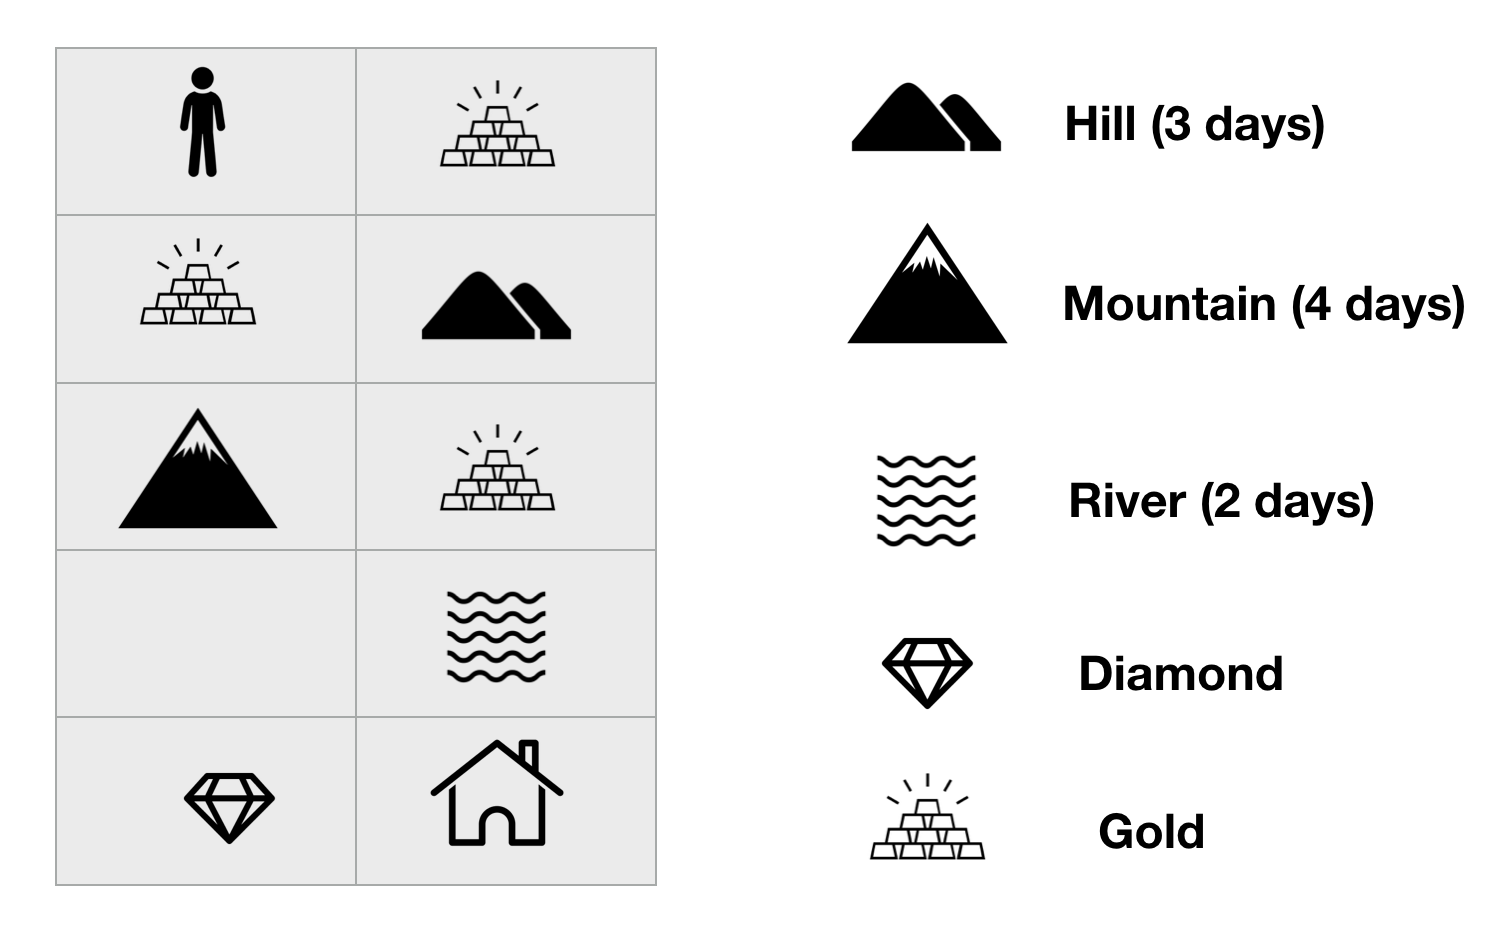
\includegraphics[width=8cm]{traveller_example}
  \caption{Traveller Problem}
  \label{fig:traveller_example}
\end{figure}

\subsection{Adaptive Program} %TODO better title?

\todo[inline]{Should the reward be from the environment? or add if statements showing how the reward is assigned?}


\begin{lstlisting}[language = Python,
                   label = {lst:abp_traveller},
                   caption = {Adaptive Program for traveller problem},
                   captionpos = b]

traveller = Adaptive(choices = [NORTH, SOUTH, EAST, WEST])

state = env.reset()

for days in range(8):
  direction_to_move = traveller.predict(state)

  state, reward, done, info = env.step(direction_to_move)

  traveller.reward(reward)

  if done:
     break

\end{lstlisting}

\todo[inline]{Is it necessary to explain the program? Or is it self explanatory?}

When the ABP program is run, the traveller decides to take the path as shown in Figure \ref{fig:traveller_decision}


\begin{figure}[h]
  \centering
  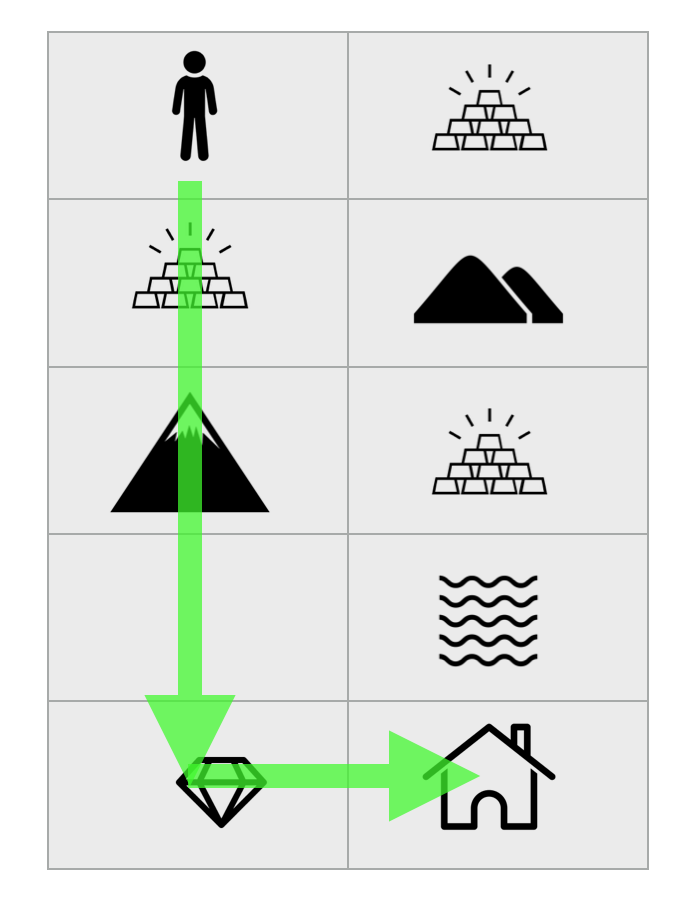
\includegraphics[height=5cm]{traveller_decision}
  \caption{Traveller Decision}
  \label{fig:traveller_decision}
\end{figure}

However it is not clear why the decision was made to take the current path. There could be several reasons
for making the decision and many unanswered questions that we can ask:
"Why did the traveller not move EAST and collect the gold on the first step?"

This can be considered as one of the disadvantages of using adaptive variables in the program.
Even though we assume the value that the adaptive variable holds is optimal, it is not clear as to why
it made the decision to hold the current value. Also making it difficult for
the programmer to debug programs containing these adaptive variables.

We explain the decisions being made by the adpative variable by extending the adpative programming library
to use reward decomposition and using predictors
\todo[inline]{Need a better way to say this! Should it be called predictors?}


\subsection{Explanation using ABP}
\todo[inline]{
1. So far we havent talked about how the adaptive variable choose its value. Is it needed? Or should it be a reference to another paper? \\
2. Need a better title \\
The goal of this sections is to make the reader understand that Q value function is a knowledge representation and has semantics
}

The adaptive variable uses reinforcement learning techniques to choose the correct value \cite{bauer2011adaptation}.
After the initial training period, the adpative variable generates a Q function \cite{bauer2011adaptation}. The value
that the adaptive variable holds is then based on the Q function. The Q function also called value function has
an explictic semantics \cite{sutton2011horde}. In the case of the traveller example it represents the knowledge of
which action to take to maximize the reward or to be more explicit which action should the traveller take to reach the
destination in 8 days and collect as much treasure as possible.
\todo[inline]{Need to rewrite this in a better way! Important concept for the paper. Elaborate more!}

\missingfigure{Show an example of traveller step with its corresponding Q value as histogram}

From the Figure it is clear that the traveller has to move south in order to maximize the reward.

However having a single Q value does not give us a sufficient explanation. It compresses the entire knowledege
of the problem into a single value. One way of getting better explanations is to decompose the Q values into
smaller Q values each representing knowledge of a particular subdomain of the problem. We propose a way of decomposing
the Q value based on the reward signals in order to generate a better explanation.

\subsection{Types for reward}
\todo[inline] {
1. Need a better title!
2. Is it reward signals or reward? Prefer reward but previous paper regard it as reward signals
Goal of this section is explain what are reward types!
}

In the traveller example described above, the reward signal could be of different types. For example, the reward
for reaching home is clearly different from the reward for finding a treasure. These reward signal have different
semantics associated with them. The traveller problem can then be decomposed into sub problems based on these reward
types. For example we can decompose the reward into 3 types for the traveller problem:
\begin{itemize}
  \item Type 1: Reward for reaching home
  \item Type 2: Reward for finding treasure
  \item Type 3: Reward related to effort of crossing terrain
\end{itemize}

Type 1 would describes the subproblem of the traveller reaching home. Type 2 would define the subproblem of traveller finding treasure.
and Type 3 is the subproblem of the traveller avoiding terrains as much of problem.

\subsection{Adaptive Program using reward types}

The adaptive program in Listing \ref{lst:abp_traveller} can be refactored to use reward types.

\begin{lstlisting}[language = Python,
                   label = {lst:abp_reward_decomposition},
                   caption = {Adaptive Program using reward decomposition for traveller problem},
                   captionpos = b]

traveller = Adaptive(choices = [NORTH, SOUTH, EAST, WEST])

state = env.reset()

for days in range(8):
  direction_to_move = traveller.predict(state)

  state, reward, done, info = env.step(direction_to_move)

  traveller.reward(reward["Home"], HOME_TYPE)

  traveller.reward(reward["Treasure"], TREASURE_TYPE)

  traveller.reward(reward["Terrain"], TERRAIN_TYPE)

  if done:
     break

\end{lstlisting}

With the refactored reward types and using Q-decomposition \cite{russell2003q} to train the
adaptive variable we have three types of Q values each containing the domain knowledge of
its own subproblem.
\todo[inline]{Should explain how reinforcement learning works for decomposed rewards?}

\subsection{Explanation using decomposed reward}
With the adaptive variable having information about the three subdomains and making its decision
based on the decomposed Q values, we can get a better explanation than before. The programmer
has more information regarding the decision of the adaptive variable.

\missingfigure{Show figure for decomposed reward}


\subsection{Example explanation}
\todo[inline]{Give an example explaining the decision of the traveller at a particular state}

\subsection{Scope of explanation}
\todo[inline]{
1.What can we explain using this method? \\
2.What are the drawbacks? w.r.t RL (discount factor), w.r.t Explanation
}

\section{Performance using reward types}


\section{Wolf Hunting Problem}
One of the issues with the approach mentioned above is that the environment may not have a single reward
type. This makes it difficult to use the approach. In order to overcome the difficulty  we introduce a
new kind of abstraction called predictors. To illustrate the use of predictors consider a simple girdworld problem consisting
of two wolves and a rabbit. The objective is for the wolves to capture the rabbit as fast a possible.
The optimal way of doing this would be for the wolves to coordinate with each other. In this case there is only one
reward type which gives the value 1 when the wolves capture the rabbit and 0 otherwise. The corresponding ABP program is shown
in the Listing \ref{lst:abp_wolf_hunt}.

\missingfigure{Show figure for wolf hunting problem}


\begin{lstlisting}[language = Python,
                   label = {lst:abp_wolf_hunt},
                   caption = {Adaptive Program for wolf hunt problem},
                   captionpos = b]

wolf1 = Adaptive(choices = [UP, DOWN, LEFT, RIGHT])
wolf2 = Adaptive(choices = [UP, DOWN, LEFT, RIGHT])

state = env.reset()

for steps in range(env.max_episode_steps):
  wolf1_action = wolf1.predict(state)
  wolf2_action = wolf2.predict(state)

  action = (wolf1_action, wolf2_action)

  state, reward, done, info = env.step(action)

  wolf1.reward(reward)
  wolf2.reward(reward)

  if done:
     wolf1.end_episode(state)
     wolf2.end_episode(state)
     break

\end{lstlisting}

\section{Explanation using ABP}

\missingfigure{Show figure for Q values for both the wolves}

\section{XABP Program}


\begin{lstlisting}[language = Python,
                   label = {lst:abp_wolf_hunt},
                   caption = {Adaptive Program for wolf hunt problem},
                   captionpos = b]

wolf1 = Adaptive(choices = [UP, DOWN, LEFT, RIGHT])
wolf2 = Adaptive(choices = [UP, DOWN, LEFT, RIGHT])

no_of_steps = Predictor()

state = env.reset()

for steps in range(env.max_episode_steps):
  wolf1_action = wolf1.predict(state)
  wolf2_action = wolf2.predict(state)

  action = (wolf1_action, wolf2_action)

  state, reward, done, info = env.step(action)

  no_of_steps.learn(state, 1, done, 0)

  wolf1.reward(reward)
  wolf2.reward(reward)

  if done:
     wolf1.end_episode(state)
     wolf2.end_episode(state)
     break

\end{lstlisting}

% needed in second column of first page if using \IEEEpubid
%\IEEEpubidadjcol

% An example of a floating figure using the graphicx package.
% Note that \label must occur AFTER (or within) \caption.
% For figures, \caption should occur after the \includegraphics.
% Note that IEEEtran v1.7 and later has special internal code that
% is designed to preserve the operation of \label within \caption
% even when the captionsoff option is in effect. However, because
% of issues like this, it may be the safest practice to put all your
% \label just after \caption rather than within \caption{}.
%
% Reminder: the "draftcls" or "draftclsnofoot", not "draft", class
% option should be used if it is desired that the figures are to be
% displayed while in draft mode.
%
%\begin{figure}[!t]
%\centering
%\includegraphics[width=2.5in]{myfigure}
% where an .eps filename suffix will be assumed under latex,
% and a .pdf suffix will be assumed for pdflatex; or what has been declared
% via \DeclareGraphicsExtensions.
%\caption{Simulation Results}
%\label{fig_sim}
%\end{figure}

% Note that IEEE typically puts floats only at the top, even when this
% results in a large percentage of a column being occupied by floats.


% An example of a double column floating figure using two subfigures.
% (The subfig.sty package must be loaded for this to work.)
% The subfigure \label commands are set within each subfloat command, the
% \label for the overall figure must come after \caption.
% \hfil must be used as a separator to get equal spacing.
% The subfigure.sty package works much the same way, except \subfigure is
% used instead of \subfloat.
%
%\begin{figure*}[!t]
%\centerline{\subfloat[Case I]\includegraphics[width=2.5in]{subfigcase1}%
%\label{fig_first_case}}
%\hfil
%\subfloat[Case II]{\includegraphics[width=2.5in]{subfigcase2}%
%\label{fig_second_case}}}
%\caption{Simulation results}
%\label{fig_sim}
%\end{figure*}
%
% Note that often IEEE papers with subfigures do not employ subfigure
% captions (using the optional argument to \subfloat), but instead will
% reference/describe all of them (a), (b), etc., within the main caption.


% An example of a floating table. Note that, for IEEE style tables, the
% \caption command should come BEFORE the table. Table text will default to
% \footnotesize as IEEE normally uses this smaller font for tables.
% The \label must come after \caption as always.
%
%\begin{table}[!t]
%% increase table row spacing, adjust to taste
%\renewcommand{\arraystretch}{1.3}
% if using array.sty, it might be a good idea to tweak the value of
% \extrarowheight as needed to properly center the text within the cells
%\caption{An Example of a Table}
%\label{table_example}
%\centering
%% Some packages, such as MDW tools, offer better commands for making tables
%% than the plain LaTeX2e tabular which is used here.
%\begin{tabular}{|c||c|}
%\hline
%One & Two\\
%\hline
%Three & Four\\
%\hline
%\end{tabular}
%\end{table}


% Note that IEEE does not put floats in the very first column - or typically
% anywhere on the first page for that matter. Also, in-text middle ("here")
% positioning is not used. Most IEEE journals use top floats exclusively.
% Note that, LaTeX2e, unlike IEEE journals, places footnotes above bottom
% floats. This can be corrected via the \fnbelowfloat command of the
% stfloats package.

\section{Conclusion}
TODO




% if have a single appendix:
%\appendix[Proof of the Zonklar Equations]
% or
%\appendix  % for no appendix heading
% do not use \section anymore after \appendix, only \section*
% is possibly needed

% use appendices with more than one appendix
% then use \section to start each appendix
% you must declare a \section before using any
% \subsection or using \label (\appendices by itself
% starts a section numbered zero.)
%


% use section* for acknowledgement
% \section*{Acknowledgment}
%
%
% The authors would like to thank...


% Can use something like this to put references on a page
% by themselves when using endfloat and the captionsoff option.
\ifCLASSOPTIONcaptionsoff
  \newpage
\fi



% trigger a \newpage just before the given reference
% number - used to balance the columns on the last page
% adjust value as needed - may need to be readjusted if
% the document is modified later
%\IEEEtriggeratref{8}
% The "triggered" command can be changed if desired:
%\IEEEtriggercmd{\enlargethispage{-5in}}

% references section

% can use a bibliography generated by BibTeX as a .bbl file
% BibTeX documentation can be easily obtained at:
% http://www.ctan.org/tex-archive/biblio/bibtex/contrib/doc/
% The IEEEtran BibTeX style support page is at:
% http://www.michaelshell.org/tex/ieeetran/bibtex/
%\bibliographystyle{IEEEtran}
% argument is your BibTeX string definitions and bibliography database(s)
%\bibliography{IEEEabrv,../bib/paper}
%
% <OR> manually copy in the resultant .bbl file
% set second argument of \begin to the number of references
% (used to reserve space for the reference number labels box)
\bibliographystyle{IEEEtran}
\bibliography{./bib/xdap}{}

% biography section
%
% If you have an EPS/PDF photo (graphicx package needed) extra braces are
% needed around the contents of the optional argument to biography to prevent
% the LaTeX parser from getting confused when it sees the complicated
% \includegraphics command within an optional argument. (You could create
% your own custom macro containing the \includegraphics command to make things
% simpler here.)
%\begin{biography}[{\includegraphics[width=1in,height=1.25in,clip,keepaspectratio]{mshell}}]{Michael Shell}
% or if you just want to reserve a space for a photo:

% \begin{IEEEbiography}[{\includegraphics[width=1in,height=1.25in,clip,keepaspectratio]{picture}}]{John Doe}
% % \blindtext
% \end{IEEEbiography}

% You can push biographies down or up by placing
% a \vfill before or after them. The appropriate
% use of \vfill depends on what kind of text is
% on the last page and whether or not the columns
% are being equalized.

%\vfill

% Can be used to pull up biographies so that the bottom of the last one
% is flush with the other column.
%\enlargethispage{-5in}




% that's all folks
\end{document}


% TODO Citations
% person by Adrien Coquet from the Noun Project
% Mountains by Aleksandr Vector from the Noun Project
% Home by il Capitano from the Noun Project
